\section{Experiments}

\begin{frame}{Experiment set up}
  \begin{itemize}
    \item \(n\) is fixed at 30M integers
    \item Sample sizes are \(10\%, 25\%, 50\%, 75\%, 90\%\) of \(n\)
    \item Run on 1-core, 12-core, and 12-core with hyperthreading
  \end{itemize}
\end{frame}

\begin{frame}{Running time of different algorithms on 1 thread}
  \begin{figure}
    \begin{center}
      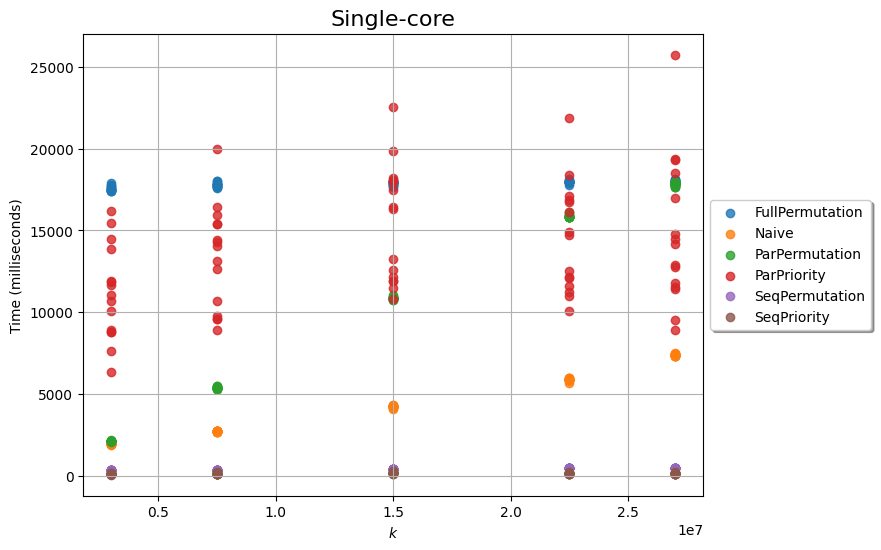
\includegraphics[height=0.8\textheight]{figures/single_core.png}
    \end{center}
  \end{figure}
\end{frame}

\begin{frame}{Running time of different algorithms on 12 threads}
  \begin{figure}
    \begin{center}
      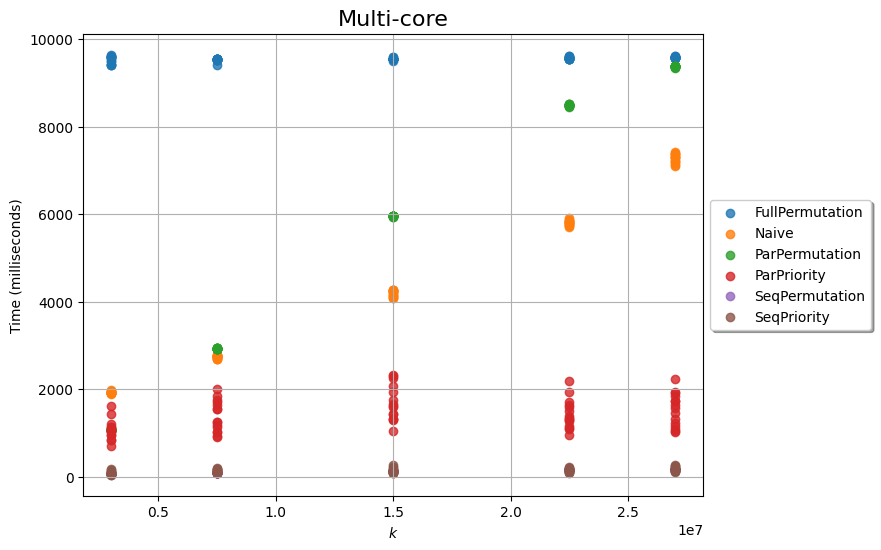
\includegraphics[height=0.8\textheight]{figures/multi_core.png}
    \end{center}
  \end{figure}
\end{frame}

\begin{frame}{Running time of different algorithms on 24 threads}
  \begin{figure}
    \begin{center}
      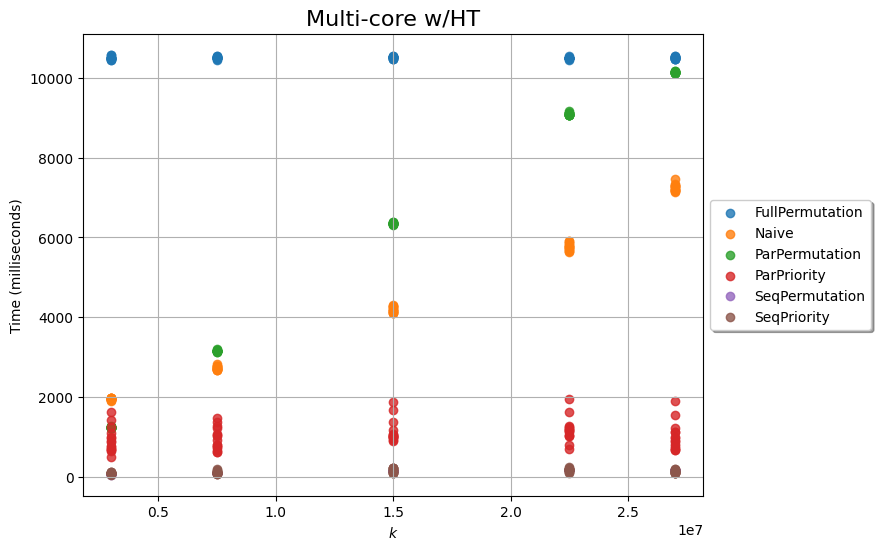
\includegraphics[height=0.8\textheight]{figures/multiht_core.png}
    \end{center}
  \end{figure}
\end{frame}
